\documentclass[11pt,a4paper]{article}
\usepackage[preset=opensansnote,title=default,pkgset=rich,par=indent]{phfnote}
\usepackage[utf8]{inputenc}
\usepackage{listings}
\usepackage{xcolor}
\usepackage{dirtree}
\usepackage[shortlabels]{enumitem}
\usepackage[german=swiss]{csquotes}
\usepackage{hyperref}

\definecolor{vs_comments}{RGB}{0,128,0}
\definecolor{vs_keyword}{RGB}{0,0,255}
\definecolor{vs_string}{RGB}{163,21,21}

% set the default code style
\lstset{
    frame=tb, % draw a frame at the top and bottom of the code block
    tabsize=4, % tab space width
    showstringspaces=false, % don't mark spaces in strings
    numbers=none, % display line numbers on the left
    captionpos=b,
    commentstyle=\color{vs_comments}, % comment color
    keywordstyle=\color{vs_keyword}, % keyword color
    stringstyle=\color{vs_string} % string color
}

\begin{document}
\title{Messerli C\# Coding Guideline}
\author{CTO Board}
\date{\today\\Version 1.0}
\maketitle

\inlinetoc

\newpage

\section{Messerli C\# coding guidelines}

These are the revised Coding Guidelines valid for code newly written in C\#.
If you see mistakes or have, comments do not hesitate in contacting the CTO-Board.

\subsection{When and where are these rules applicable}

These rules are applicable to all C\# code written at Messerli Informatik AG. 
The rules will not be enforced for old code, which has not been changed.
In a review, these coding guidelines should be checked for all code, which has changed.
Changes necessary due to the coding guidelines should be in a reasonable ratio to the functional changes.

\subsection{Update to the rules and glossary}

Updates to the rules and glossary should be sent to the CTO-Board. The CTO-Board will integrate new rules or new words in the glossary in a timely fashion when the board approves and will give feedback otherwise.

\subsection{Definition of done}

Code builds without new warnings

\begin{itemize}[itemsep=0pt]
  \item Feature is tested against acceptance criteria
  \item Code adheres to the Coding Guidelines
  \item Unit tests pass
  \item Code is unit tested
  \item Code is reviewed
\end{itemize}

\section{Physical structure}

\subsection{Each class should go into its own file with the same name}

Only one class should be in a file. This also applies to Enumerations.
Inner classes are allowed but discouraged and an obvious exception to this rule. 

\subsection{Each namespace should go into its own folder with the same name}

All classes that are held together by a common purpose should go into its own namespace; the namespace should be reflected in the folder structure. If you have a namespace Example, it should be in a folder example.
Set a correct default namespace in the project, this way the tooling will help you to move classes into the correct location.

\subsection{Each project should have a test project}

We write tests in a separate project, therefore each project needs a test-project.

\section{Formatting rules}

We use Visual Studio, ReSharper and CodeMaid to enforce most of the formatting rules. 

\subsection{Tool configurations}
The Formatting Rules for Visual Studio, ReSharper and CodeMaid are checked into the Repository, and can be found in the CTO git-Repository in the folder Tool Configurations:
\begin{itemize}[itemsep=0pt]
  \item .editorconfig
  \item CodeMaid.config
  \item MesserliResharper.DotSettings
  \item VS\_Format\_Settings.vssettings
\end{itemize}

\subsection{Indentation}

For each scope that is opened, we indent by one level.
For indentation, we use only spaces, tabs are forbidden.
One level of indentation is four spaces.

\subsection{Maximum line length}

There is no absolute maximum to the length of the line, but try to keep it on the screen.

\subsection{Empty lines}

We use only one empty line to separate content.

\section{Naming conventions}

Names should be descriptive; avoid abbreviations.
Give a descriptive name, but be specific. Do not worry about saving horizontal space, as it is far more important to make your code immediately understandable by a new reader. We do not contract words or make up words.

\subsection{We use English words for abstractions}
\begin{itemize}[itemsep=0pt]
  \item The programming language is in English, most concepts are in English, therefore English is a lot easier to make consistent. (WriteExportAbacusEinFile, etc.)
  \item Most of the concepts except a few in the building industry are already in English.
  \item We want to avoid being confused about GetProject vs GetProjekt. For a single concept, only one word in one language should be chosen.
  \item Avoid variables like workWork (sic)
  \item It is a lot easier to create plurals in English (-s, -ies) where in German it might be difficult: Kapitel, Mitarbeiter, Unternehmer, Fenster, Artikel (see also next point)
  \item Proper Nouns  should not be translated even if possible.
  \item We try to use the same word for the same abstraction. It is either a project or a tenant. (DDD)
  \item All widely used concepts should be listed in the glossary
\end{itemize}

\subsection{Be specific}

 
\begin{figure}[ht]
  \centering
  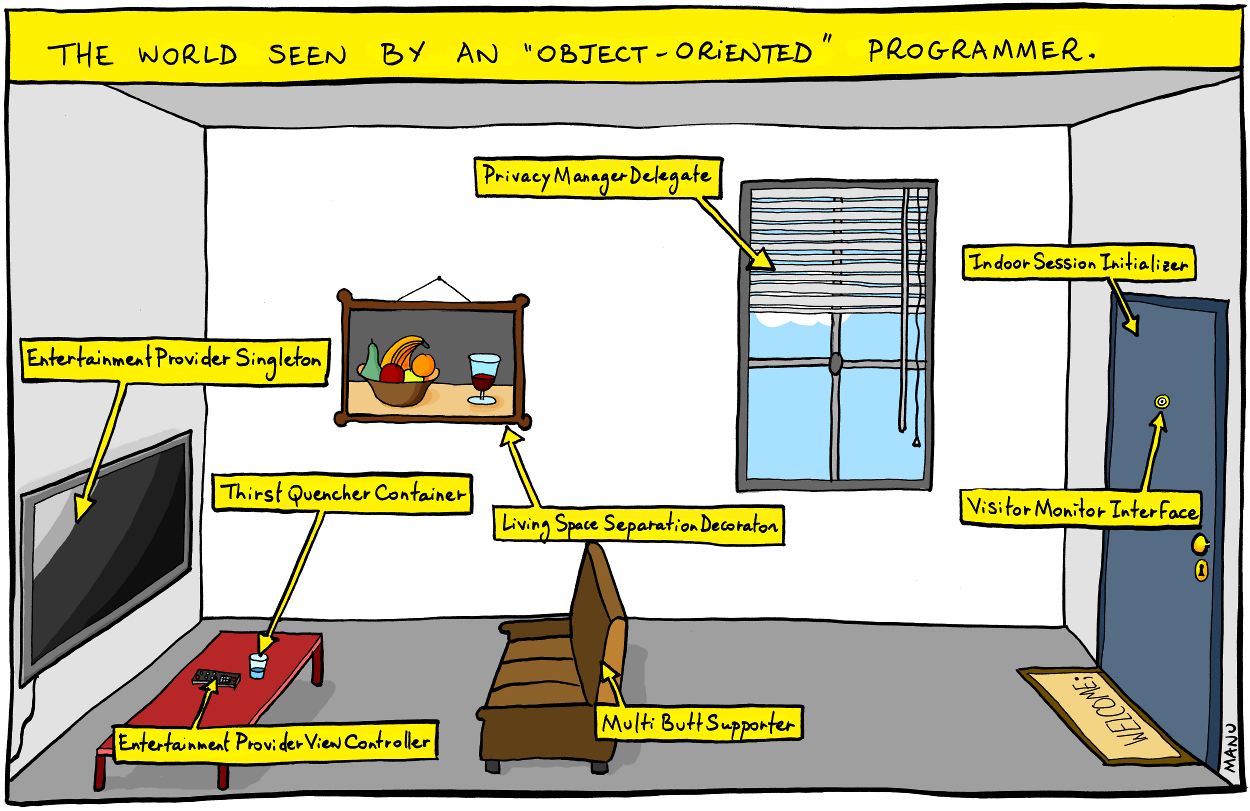
\includegraphics[width=0.7\textwidth]{oop-naming.png}
  \caption{!DDD}
\end{figure}

Only use generic words like, data, list, string, number, manager, gateway and handler if necessary in a generic context. Otherwise, try to find specific domain words. Build a domain specific ubiquitous language.
In domain context, always use the domain vocabulary and try keeping the overhead to a minimum, be precise.

\subsection{Abbrevations}
We do not use abbreviations that are ambiguous or unfamiliar to readers outside our project, and we do not abbreviate by skipping letters within a word. Abbreviations that would be familiar to someone outside your project with relevant domain knowledge are OK. As a rule of thumb, an abbreviation is probably OK if it is listed in Wikipedia like IP or HTML.
All abbreviations are written in PascalCase.

\begin{lstlisting}[language={[Sharp]C}, caption={Abbrevation Examples}]
class JsonToHtmlConverter {}
class IpAddress {}
class UserId {}
class TfsConnector {}
\end{lstlisting}

\filbreak

\subsection{Use plural and singular to your advantage}
If you have a collection of things, use the plural form of the variable you would use for a single element. Prefer being specific, as the name of the collection should reflect the meaning behind its elements. This gives you a natural understanding on what object you are dealing with.

\begin{lstlisting}[language={[Sharp]C}, caption={Correct usage of plural}]
var onlineUsers = GetOnlineUsers();
for (var user in onlineUsers) {
    user.GoOffline();
}
\end{lstlisting}

\subsection{Try to use the same word for the same concept}

Do not switch between different name for a concept, make a choice and stick to it.

\subsection{Naming the different C\# identifiers }

Table \ref{naming_identifiers} gives you the rules for each identifier.

\begin{table}
\centering
\begin{tabular}{lp{20mm}p{25mm}l}
 \textbf{Identifier} & \textbf{Casing} & \textbf{Prefix / Suffix} & \textbf{Example} \\
  \hline
 Namespace                 & PascalCase &                 & Messerli.Core            \\
  \hline
 Class                     & PascalCase &                 & WarpEngine               \\
  \hline
 Exception class           & PascalCase & <Name>Exception & InvalidArgumentException \\ 
  \hline
 Interface                 & PascalCase & I<Name>         & ISyntaxTree              \\
  \hline
 Abstract class            & PascalCase &                 & Application              \\
  \hline
 Method                    & PascalCase &                 & DrawSquare               \\
  \hline
 Properties                & PascalCase &                 & FirstName                \\
  \hline
 Predicate method          & PascalCase & Is<Name>, Has<Name>, Are<Name>, Have<Name> & IsGreat, HasField \\
  \hline
 Public Member Variable    & PascalCase &                 & Diameter                 \\
  \hline
 Protected member variable & camelCase  & \_<name>        & \_tableIndex             \\
  \hline
 Private member variable   & camelCase  & \_<name>        & \_adjacencyMatrix        \\
  \hline
 Local variable            & camelCase  &                 & index, name, helpLabel   \\
  \hline
 Global constant           & PascalCase &                 & Pi, PrimeNumbers         \\
  \hline
 Class constant            & PascalCase &                 & FilePath                 \\
  \hline
 Enum type                 & PascalCase &                 & StatusType               \\
  \hline
 Enum value                & PascalCase &                 & RequiredValue            \\
  \hline
 Lambda Parametrs          & camelCase \newline lower-case letter  & & cornerPoint, c, name, n    \\
\end{tabular}
\caption{Naming rules}
\label{naming_identifiers}
\end{table}

\subsection{UI Elements}
When dealing with UI Elements like buttons, combo boxes, grids, text boxes, etc. we append the full name of the type without any prefix to the variable name. 

\begin{lstlisting}[language={[Sharp]C}, caption={Naming of UI Elements}]
class UserRightDialog {
    Grid _userGrid;
    Edit _userNameEdit;
    Button _okButton;
};
\end{lstlisting}

\subsection{Naming of delegate variables}

All delegate variables should be in camelCase without a prefix or postfix. All other Methods are PascalCase which means if you see a createThing(), you will know that it is indeed a delegate call.

\subsection{Naming of Tests}

The naming of tests must describe what the intended effect of the methods that are being tested, e.g. `ReturnsNullOnEmptySettings` or `ThrowsOnInvalidResponse`

\section{Variables}

\subsection{Only one declaration per line}

Multiple declarations per line are not allowed. This way, we can reduce the mental baggage of the reader and avoid awkward pointer and reference declarations (See the next subchapter).
Deconstruction of Tuples and other types are obviously exempt from this rule. 

\begin{lstlisting}[language={[Sharp]C}, caption={Example: tuple deconstruction}]
var (name, address, city, zip) = contact.GetAddressInfo();
\end{lstlisting}

\subsection{Local variables have good names}

Local variables should have self-evident names too. Every variable should describe its content, and named consistently. One can often reuse the name of the type. Be as specific as necessary and as short as possible.

\subsection{Declare variables in the innermost scope that is possible}

This rule attempts to minimize the number of live variables that must be simultaneously considered. Furthermore, variable declarations should be postponed until enough information is available for full initialization. This rule also reduces the possibility of uninitialized and wrongly initialized variables.

\subsection{Define variables on declaration}

Local variables of primitive type are not initialized. Try to avoid separation of declaration and definition.

\begin{lstlisting}[language={[Sharp]C}, caption={Bad example}]
// Do not write this!
Money money;
money = GetMoney();
\end{lstlisting}

\begin{lstlisting}[language={[Sharp]C}, caption={Better example}]
Money money = GetMoney();
\end{lstlisting}

\begin{lstlisting}[language={[Sharp]C}, caption={Even better example}]
var money = GetMoney();
\end{lstlisting}

This can lead to problems if your variable is initialized differently on a certain condition (if/switch). Prefer the use of if-expressions with the the ternary operator (? :) for simple cases or extract the initialization into a function

\begin{lstlisting}[language={[Sharp]C}, caption={This could also be easily refactored into a function}]
var money = HasBank() 
    ? GetFromBank() 
    : GetCash();
\end{lstlisting}

This not only avoids uninitialized variables, but makes sure you always handle both cases.

With C\# 8.0 switch-expressions are introduced which are highly recommended instead of switch-statements.

\subsection{Do not reuse variables}

A variable should have only one single purpose; there is no reason to recycle variables. The variables are abstractions for the human reader and not memory locations for the compiler.

\subsection{Prefer type inference}

Use var to avoid type names, especially those that are noisy, obvious, or unimportant — cases where the type does not aid in clarity for the reader. Only use manifest type declarations when it helps readability.

\begin{lstlisting}[language={[Sharp]C}, caption={Type inference}]
var textBox = GetTextBox();
textBox.SetText("foo");
\end{lstlisting}

This does not mean that you should blindly replace types with var.

\subsection{Do not use magic values}

Every number except 0 or 1 needs a useful name derived from its true meaning in the code. However, this does not mean that 0 and 1 cannot have a name too.
The same goes for magic strings!

\subsection{Unused variables with discared values}

Ideally we would prefer a clean way with pattern matching, where we always could use \_. Since this is only possible in certain parts of the language, we still try to use the \_ for unused variables. If you have more than one unused variable in the same context, use \_0, \_1, ... instead.

\section{Basic constructs}

\subsection {Only one expression per line}

Multiple expressions or statements in one line increase the mental burden while reading them. Split them up to avoid mentally hiding statements.

\subsection{Prefer logical operators to if statements}

\begin{lstlisting}[language={[Sharp]C}, caption={Avoid if and ternary operator for logical expressions}]
if (node.GetParenthesis(key)) {
    item.Setting = false;
} else {
    item.Setting = true;
}
\end{lstlisting}

Logical expressions have no branches, are more concise and always handle all the logical cases.

\begin{lstlisting}[language={[Sharp]C}, caption={Use logical operators !, \&\& and ||}]
item.Setting = !GetParenthesis(key);
\end{lstlisting}


\subsection{If-statements}

The condition of the if-statement should have no side effects.
Avoid nested if-statements and prefer logical operators.

\begin{lstlisting}[language={[Sharp]C}, caption={Avoid side-effects}]
    if (!Move(id)) {
        return false;
    }

    if (!UpdateStart(StartValue)) {
        return false;
    }
\end{lstlisting}

\begin{lstlisting}[language={[Sharp]C}, caption={Better alternative}]
    var itemFound = Move(id);
    if (!itemFound) {
        return false;
    }

    var updateIsReady = UpdateStart(StateDelete);
    if (!updateIsReady) {
        return false;
    }
\end{lstlisting}

\subsection{ternary operator}

Prefer the ternary operator to simple if statements. The ternary operator is an expression in contrast to the if-statement and it forces you to handle all the cases.

We format the ternary operator like this, to see which branch we are dealing with easily.

\begin{lstlisting}[language={[Sharp]C}, caption={ternary operator}]
    return condition
        ? true-expression
        : false-expression;
\end{lstlisting}

\subsection{switch expression}

Prefer switch expression over switch statements.

\begin{lstlisting}[language={[Sharp]C}, caption={switch expression}]
    return animalKind switch
    {
        AnimalKind.Dog => "dog",
        AnimalKind.Cat => "cat",
        _ => throw new InvalidOperationException(
          $"Unsupported animal kind {animalKind}"),
    };
\end{lstlisting}

\subsection{For-loops}

Avoid for-loops and use LINQ and higher order functions as an alternative.

\subsubsection{Prefer foreach-loops}

Whenever you are iterating over some kind of enumerator, prefer the foreach syntax:

\begin{lstlisting}[language={[Sharp]C}, caption={foreach-loop}]
foreach (var value in values.OrderByDescending(v => v)) {
    // Do something in reverse order
}
\end{lstlisting}

\subsection{Switch-statement}

\subsubsection{Handle all cases}

Unhandled cases lead the program into an undefined state. If you have no natural default case, declare one throwing a System.NotImplementedException.

\subsection{Goto}

The goto statement is forbidden in all cases.

\section{Types}

\subsection{Use strong types}

C\# has a strong typing system, take advantage of it. A strong type will help you a lot in refactoring, and the compiler will easily tell you that you are using the wrong parameter if you do not have a string type like a comma separated list instead of a strong collection like a vector of longs.

\begin{lstlisting}[language={[Sharp]C}, caption={Create a strong type}]
class Vector {
    int X;
    int Y;
    int Z;
}

Vector CrossProduct(Vector factor1, Vector factor2);

// Never do this
bool CrossProduct(long x1, long y1, long z1, long x2, long y2, long z2,
                  out long resultX, out long resultY, out long resultZ);
\end{lstlisting}

\subsubsection{New type idiom}
The idea behind the new type idiom is to have additional type information, even if you have a single integer as an argument. Even when we have simple integers, it usually represents a concept not as generic. This concept could be years, bytes, money or position. 
 So even if you have a single integer, you can create a new type from your abstract concept.

\begin{lstlisting}[language={[Sharp]C}, caption={Declaring the new type Years}]
    class Years {
        Years(int years)
        {
            Value = years;
        }

        int Value { get; }
    }
\end{lstlisting}

In this case we have a time period in years. The constructor should be explicit, otherwise a Year object would be automatically constructed from a given integer. That way you need to be explicit when you call a function like this:

\begin{lstlisting}[language={[Sharp]C}, caption={Use the new type}]
bool OldEnough(Years years)
\end{lstlisting}

The Function OldEnough only accepts years. If you give an integer or a value of type Days you will get a compilation error. This helps in self-documentation and avoids misunderstandings between programmers with different assumptions. The code the compiler produces is the same with or without the additional type information. The additional Type-Information is just a compile time hint for the programmer.

\subsubsection{Do not convert the types from the API if not necessary}

Casting types can lead to unexpected behavior and should be avoided, if you need to convert types, chose a place where it minimizes the number of casts.

\subsection{Define appropriate types}

If two or more items of data belong together, try to find a name for them, and define a type you can reuse. Only use Tuple when the data is generic or part of an external interface.

\subsection{Use appropriate data-structures}

Do not pass around data structures as strings or tuples, when you could create a better type for your data.

\subsection{Use Readonly PODs for data}

All PODs must inject their state in the constructor and provide read only properties to it.
A public setter is forbidden, a private setter is discouraged. 

\subsection{Make PODs easy to use}

PODs should implement IEquatable or IComparable, use Fody instead of manual implementation if possible.

\section{Functional Programming}

\subsection{Immutability}

While only data can have side effects, it is the methods and functions, which profit the most of immutability. They are much easier to understand and usually the code is much more elegant when you stay away from mutability. A function f in program P has no side-Effect if f() == f() for all states of P. In addition, the state of P does not change if you invoke f.
Programs without side effects are easy to test because it implies that any test of f is independent of the state of P.

\subsubsection{Prefer immutable types to mutable ones}

An immutable type can only set its state through a constructor. No stateful setters are allowed on an immutable type. Changing state is done through transformation by copying. This way, even a setter can be written in an immutable way:


\subsection{Use higher-order functions with LINQ and avoid writing your own for-loops}

We try to avoid unnecessary repetition. For many things, there are generic algorithms. Use LINQ and other Algorithms to create powerful abstractions.
If there is not an algorithm available, try to be generic and write your own algorithms.

\begin{table}
\centering
\begin{tabular}{lp{60mm}l}
\textbf{Task}        & \textbf{LINQ}                                         \\
\hline
Projection           & Select, SelectMany                                    \\
\hline
Aggregation          & Aggregate, Sum, Min, Max, Average, Count              \\
\hline
Restriction          & Where                                                 \\
\hline
Existence            & Any, All, Contains, Distinct                          \\
\hline
Set Operations       & Contains, Distinct, Union, Intersect, Except          \\
\hline
Sorting              & OrderBy, ThenBy, OrderByDescending, ThenByDescending  \\
\hline
Paging               & First, Last, Single, Skip, Take, SkipWhile, TakeWhile \\
\hline
String Formating     & string.Format() or use \$"" (String interpolation)
\end{tabular}
\end{table}

\subsubsection{LINQ syntax}

Extension Methods and LINQ syntax are equivalent. Both have their up- and down-sides. Chose the one which you think is most appropriate for the Task at hand. You can also mix them in the same code file if it makes the code easier to read.

\subsection{Use the import of static functions to your advantage}

With the ability to import static functions, the syntax is much more natural to call functions on their own. Use that to your advantage and write free functions independent of any type.

\section{Object oriented programming}

\subsection{Abstraction}

\subsubsection{Depend on abstractions not implementations}

Classes which are not PODs must depend on abstractions and not implementations if possible.

\subsubsection{Create your own abstractions if none are available}

If the library you are using do not offer their own abstractions, create a facade with your own abstractions in front of the implementation.

\subsubsection{Factories}

Avoid the usage of new, either inject types through the constructor or use factories to create objects on runtime. All Factories should be declared via a delegate in the form of Listing \ref{factory_signature};

\begin{lstlisting}[language={[Sharp]C}, caption={Signature of factories},label={factory_signature}]
public delegate ReturnValue ReturnValueFactory(Parameters parameters)
\end{lstlisting}


\subsection{Inheritance}

\begin{itemize}[itemsep=0pt]
    \item If the relation between two entities can be described as a \enquote{Entity A has B}-relation then composition is to be used. You should only use inheritance if you are dealing with a \enquote{Entity A is a kind of B}-relation. See: Composition over inheritance.
    \item Prefer inheriting from interfaces
    \item Keep your inheritance hierarchy flat
		\item avoid abstract classes
\end{itemize}

\subsection{Encapsulation}

\subsubsection{Data-Members are by default private}

Classes are meant to hide the implementation details; this also means that your data should be hidden from the outside. If you really need public data-members, you might want to think about separating the data into a POD class.

\subsubsection{Use the most restricitive visibility modifier possible}

Information should be encapsulated as much as possible, which means in first instance it should be private.

\subsubsection{public fields are forbidden}

We only use properties for public interfaces for PODs and other classes.

\subsection{Polymorphism}

\subsubsection{Use the strategy Pattern for different implementations of the same algorithm}

The strategy pattern embodies two core principles of object-oriented programming, it encapsulates the concept that varies and lets programmers code to an interface, not an implementation.

\subsubsection{Use the different forms of polymorphism to your advantage}

C\# supports runtime subtype polymorphism with virtual Methods, but there are other forms of polymorphism in C\#.

The other form is the ability to overload methods with different parameter types which is a form of static compile time polymorphism. It is more powerful in the regard that you can overload on any type and you do not need to have a type hierarchy for it to work. However be careful on this, the overload resolution uses the static type-definition and not the run-type type definition. Which means this is limited to cases where you exactly know the type at compile time.

\subsubsection{Use the visitor pattern for double dispatch}

\href{https://eli.thegreenplace.net/2016/a-polyglots-guide-to-multiple-dispatch/}{Static overload resolution can dispatch on more than one type}, but at runtime we are limited to a single dispatch mechanism offered by the subtype polymorphism. To overcome this, we need to take advantage of both forms of polymorphism offered in C\#. The visitor pattern is the right choice in such cases.

\section{Methods}

\subsection{Usually keep a method signature on one line}

Alternativly get each parameter on a single line, especially for constructors where the injected objects can change often.

\begin{lstlisting}[language={[Sharp]C}, caption={Function signature}]
void Signature(int foo, CString bar);
\end{lstlisting}

\subsection{Write short methods}

Prefer small and focused functions.
We recognize that long functions are sometimes appropriate, so no hard limit is placed on functions length. If a function exceeds about 30 lines, think about whether it can be broken up without harming the structure of the program.
Even if your long function works perfectly now, someone modifying it in a few months may add new behavior. This could result in bugs that are hard to find. Keeping your functions short and simple makes it easier for other people to read and modify your code.
You could find long and complicated functions when working with some code. Do not be intimidated by modifying existing code: if working with such a function proves to be difficult, you find that errors are hard to debug, or you want to use a piece of it in several different contexts, consider breaking up the function into smaller and more manageable pieces.

\subsection{Output parameters}

Output parameters are forbidden. They are bad style and not necessary. Return multiple values as a tuple or your own better datastructure.

\begin{lstlisting}[language={[Sharp]C}, caption={Multiple return values}]
(ReceiverChannel,SendingChannel) CreateChannels();
var (rx, tx) = CreateChannels();
\end{lstlisting}

\subsection{Ref parameters}

Ref parameters are forbidden in our own API.

\section{Namespaces}

Nothing should be in the global namespace.

\begin{itemize}[itemsep=0pt]
  \item The first level namespace is Messerli
  \item The second level namespace reflects the module you are working in
\end{itemize}


\section{Exceptions}

Exceptions are a good tool to signal behavior out of the ordinary.

\subsection{Use Nullable (?) types if you need to represent values with a no-value state}

Do not use bools to indicate illegal state, as they can easily be ignored. Wrapping a returned type in an nullable value forces the caller to check for the state. Ideally use them in a monadic way with an appropriate library.

\subsection{Do not use exceptions for control flow}

Exceptions should be used to signal exceptional behavior, such as incorrect user input or missing resources. Using them for (expected) control flow is analogous to using a goto statement.

\section{Miscellaneous}

\subsection{Use the Humble Object Pattern for System boundaries like UI}

At the boundaries of the system, where things are often difficult to test use the humble object pattern to make it better testable. We accomplish the pattern by reducing the logic close to the boundary, making the code close to the boundary so humble that it doesn't need to be tested. The extracted logic is moved into another class, decoupled from the boundary which makes it testable.

\subsection{Use the type system}

Unit tests became extremely popular with dynamically typed languages like Ruby and JavaScript out of necessity. Those languages became popular initially for relatively small code fragments for automation or simple tasks. They were not designed as system languages with millions of lines of code in mind. But these languages became popular and the ecosystem grew and therefore also the need for refactoring in bigger projects. Since the type system were weak the compiler or run-time could not help much in finding defects. 
Unit tests do much more than just checking if the types are in the expected range, and if a function is correctly typed, but it is one kind of unit tests we do not need in statically typed languages. However it is important that you actually use the type System to your advantage.

\subsection{Avoid regions}

Regions can distract and hide things from you, that is why regions are generally discouraged except for automatically generated code, you wouldn't want to change by hand.

\section{Comments}

Though a pain to write, comments are vital to keeping our code readable. The following rules describe what you should comment and where. However, remember: while comments are very important, the best code is self-documenting. Giving sensible names to types and variables is much better than using obscure names that you must then explain through comments.
When writing your comments, write for your audience. The next contributor who will need to understand your code. Be generous - the next one may be you!

\subsection{Language}

Comments are written in English.

\subsection{Style}

We only use double and triple-slash comments. We do not use the /* */ - style comments.
Write your comments above your code you want to comment. Only write comments on the right side of the code when doing so would benefit the readability greatly and the code in question is very short, e.g. an initialization.
If your code describes a block of code, consider refactoring it into a function.

\subsection{XML comments}

Try to document your public interface. 

\begin{itemize}[itemsep=0pt]
    \item The comments for an interface should be only in the header file.
    \item Try avoiding stating the obvious.
    \item We use XML-comments to document the interface.
\end{itemize}

\begin{lstlisting}[language={[Sharp]C}, caption={Commenting a function}]
/// <summary>
/// Disconnects a previously connected slot
/// </summary>
/// <param name="slotId">id of the slot</param>
void Disconnect(int slotId); 
\end{lstlisting}

We want to adhere closely to this style because Visual Studio can read and interpret the XML comments, and IntelliSense will give you a real-time information on ctrl-space. As you can see, you do not only get the general summary, but a value-by-value reference of the parameters.

\subsection{Write useful comments}

A comment is useful, if it helps to understand the code better than without. Comments are not useful if they state the obvious or are repeating what the code already tells you.
Comments are especially useful if you do something out of the ordinary, or complex. A high-level description of an algorithm for example is usually a good idea.

\subsection{ASCII Art seperators are forbidden in code}

For visual seperation you can use a \#pragma region declaration.

A region can be folded for increased visibility:

\begin{figure}[ht]
  \centering
  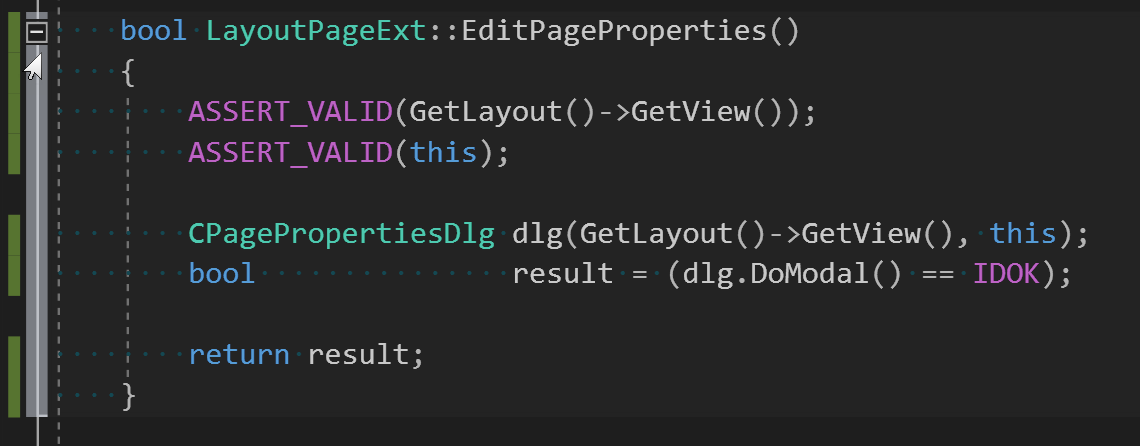
\includegraphics[width=0.7\textwidth]{pragma-region-open.png}
  \caption{Define a region}
\end{figure}

\begin{figure}[ht]
  \centering
  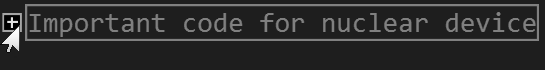
\includegraphics[width=0.7\textwidth]{pragma-region-closed.png}
  \caption{Region folded}
\end{figure}
    
\subsection{Comments on curly brace}

There are no comments on the ending curly brace. Your IDE can do code folding

\begin{figure}[ht]
  \centering
  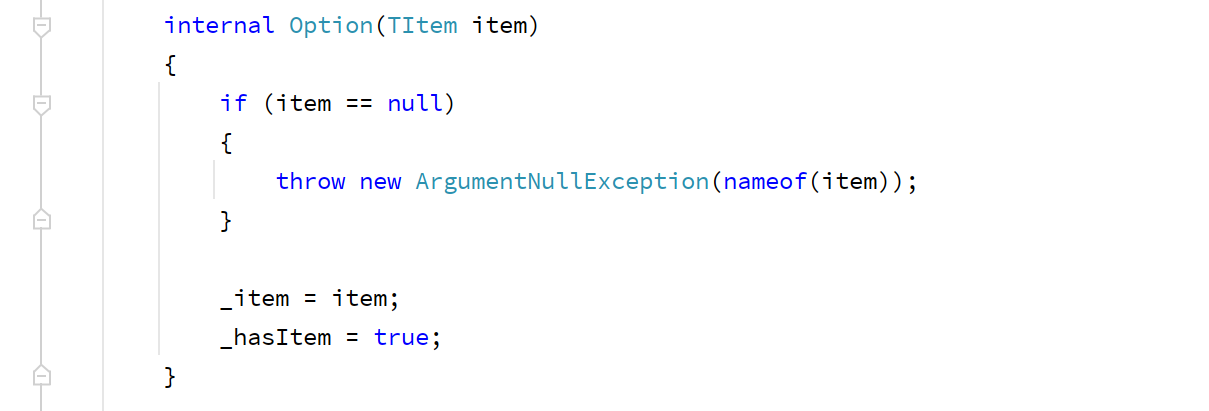
\includegraphics[width=0.7\textwidth]{code-folding-open.png}
  \caption{Function not folded}
\end{figure}

\begin{figure}[ht]
  \centering
  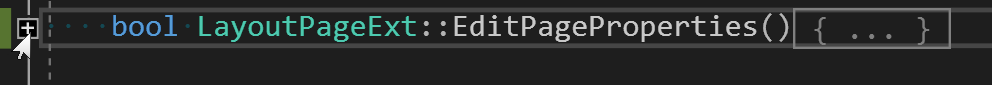
\includegraphics[width=0.7\textwidth]{code-folding-closed.png}
  \caption{Function folded}
\end{figure}

\subsection{Do not commit code that is commented out}

Code that is not compiled will rot and will be useless soon. If you really need the code, why is it not compiled? Delete the code. If you really need it again, you can always use your source control system.

\section{Commit Message}

We follow six of the seven rules of great commit messages

\begin{enumerate}
  \item Separate subject from body with a blank line
  \item Limit the subject line to 50 characters
  \item Capitalize the subject line
  \item Do not end the subject line with a period
  \item Use the imperative mood in the subject line 
  \item Use the body to explain WHAT and WHY vs. HOW
\end{enumerate}

Commit messages are written in English
\newline
The rule \enquote{Wrap the body at 72 characters} does not apply to TFVC users, as Visual Studio takes care of wrapping the body correctly.
In addition, we prepend the commit message with the module that has been worked on, followed by a colon. This prefix does not count towards the subject line character limit.
\newline
\textbf{Bad example}: Added feature
\newline
\textbf{Good example}: Document Editor: Add copy-pasting feature
\newline
\textbf{Bad example}:  A position with a parts list can be inserted in your own parts list, which leads to a program crash.
\newline
\textbf{Good example}: Catalag: Fix Crash happening in recursive parts list
A position which had itself a parts list could wrongly be inserted into a parts list.

\end{document}